\subsection{Additional functions}

\begin{frame}{Additional functions: graphical summary}
    \begin{itemize}
        \item \textbf{Box-plot:} graphical summary of the distribution of simulations results
    \end{itemize}
    \begin{figure}[t]
        %\centering
        \textbf{compositionPop2()}\par\medskip
        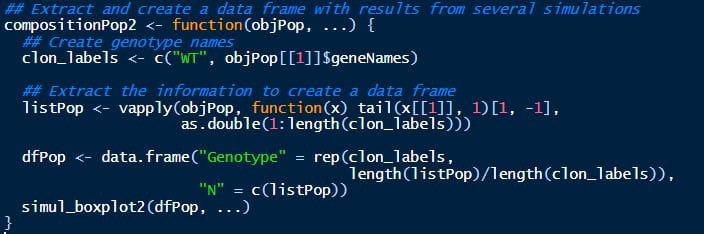
\includegraphics[width=0.8\linewidth]{img/compositionPop2.PNG}
        \caption{Code for compositionPop2() function}
    \end{figure}
\end{frame}

\begin{frame}{Additional functions: graphical summary}
    \begin{figure}[t]
        %\centering
        \textbf{simul\_boxplot2()}\par\medskip
        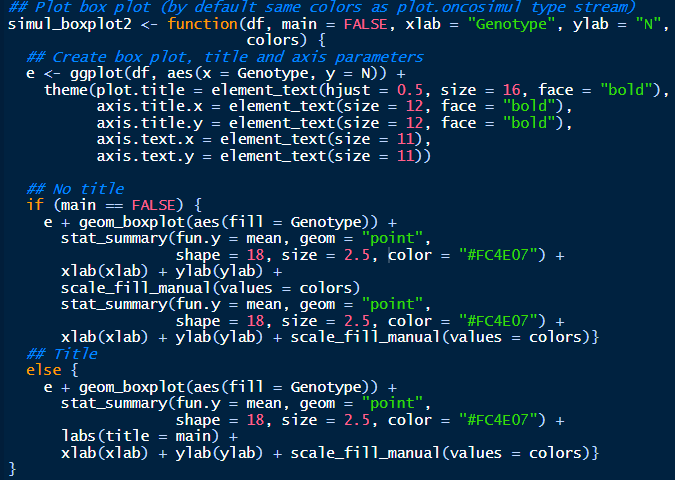
\includegraphics[width=0.7\linewidth]{img/simul_boxplot.PNG}
        \caption{Code for simul\_boxplot2() function}
    \end{figure}
\end{frame}

\begin{frame}{Additional functions: graphical summary}
    \begin{figure}
    %\centering
    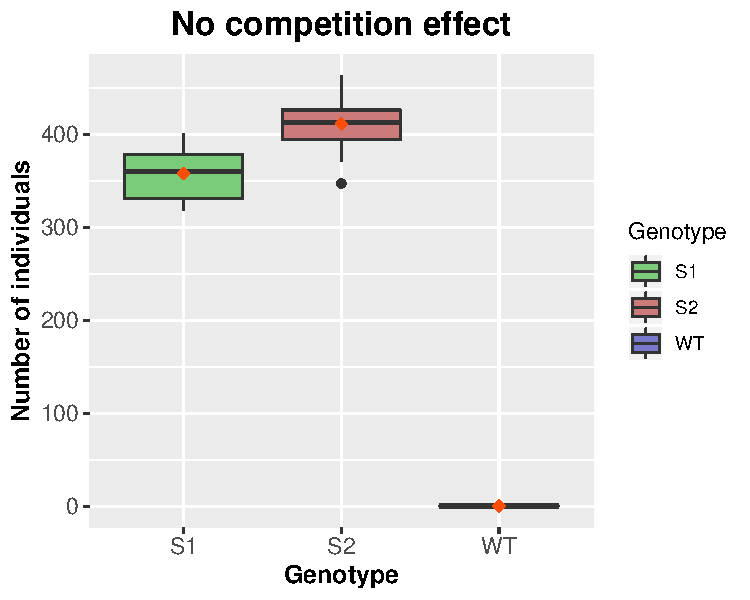
\includegraphics[width=0.7\linewidth]{img/boxplot_example.pdf}
    \caption{Box-plot from one of the Lotka-Volterra's example. 20 simulations were made.}
    \end{figure}
\end{frame}

\subsection{Modification of the code}

\begin{frame}{Modification of the code}
\begin{itemize}
        \item \textbf{Legend}
\end{itemize}
\begin{columns}
        \begin{column}{0.5\textwidth}
            \begin{figure}[t]
                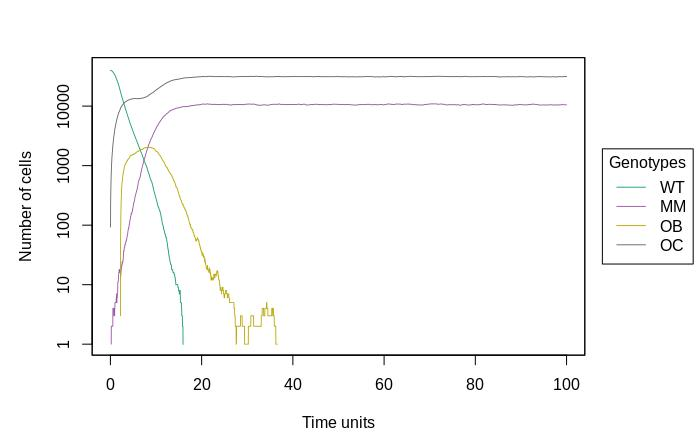
\includegraphics[width=0.9\linewidth]{img/scenario1_tr.jpg}
            \end{figure}
        \end{column}
        \begin{column}{0.5\textwidth}
            \begin{figure}[t]
                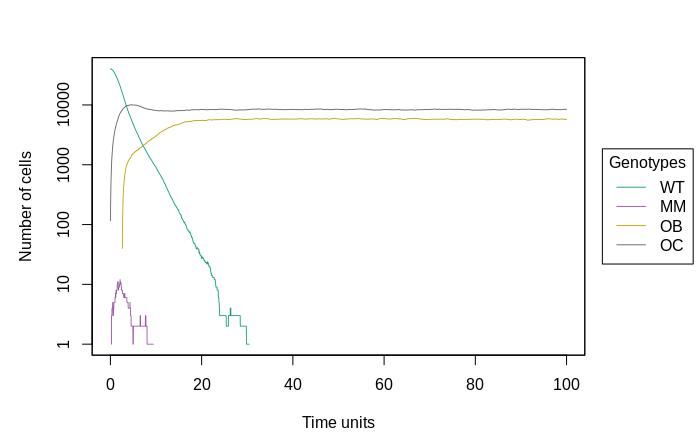
\includegraphics[width=0.9\linewidth]{img/scenario2_tr.jpg}
            \end{figure}
        \end{column}
    \end{columns}
\end{frame}